\documentclass[11pt,reqno,a4paper]{amsart}
\usepackage{amssymb,amsmath}
\usepackage{tikz,tikz-cd}
\usetikzlibrary{calc}
\usepackage{hyperref}\hypersetup{colorlinks=true, linkcolor=purple, citecolor=blue}

\begin{document}

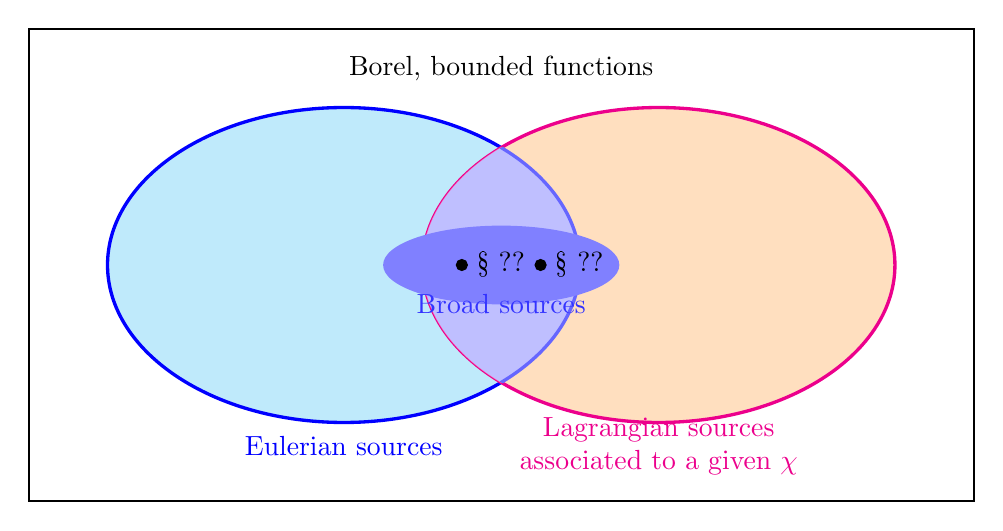
\begin{tikzpicture}
% Outer rectangle
\draw[thick] (0,0) rectangle (12,6);
\node[align=center] at (6,5.5) {Borel, bounded functions};

% Left circle - Eulerian sources
\filldraw[color=blue, fill=cyan!25, very thick](4,3) circle (3 and 2);
\node[text=blue, align=center] at (4,0.7) {Eulerian sources};

% Right circle - Lagrangian sources
\filldraw[color=magenta, fill=orange!25, very thick](8,3) circle (3 and 2);
\node[text=magenta, align=center] at (8,0.7) {Lagrangian sources\\associated to a given $\chi$};

% Intersection - Broad sources
\begin{scope}
  \clip (4,3) circle (3 and 2);
  \filldraw[color=magenta!60, fill=magenta!25](8,3) circle (3 and 2);
\end{scope}

\begin{scope}
  \clip (8,3) circle (3 and 2);
  \filldraw[color=blue!60, fill=blue!25, very thick](4,3) circle (3 and 2);
\end{scope}

% Ellipse for "Broad sources"
\fill[blue!50] (6,3) ellipse (1.5 and 0.5);
\node[text=blue!80!white, align=center] at (6,2.5) {Broad sources};

% Points with section references
\filldraw (5.5,3) circle (.07) node[right=2pt] {§ ??};
\filldraw (6.5,3) circle (.07) node[right=2pt] {§ ??};

\end{tikzpicture}

\end{document}